\documentclass[tikz,border=3pt]{standalone}
\usetikzlibrary{intersections}

\begin{document}
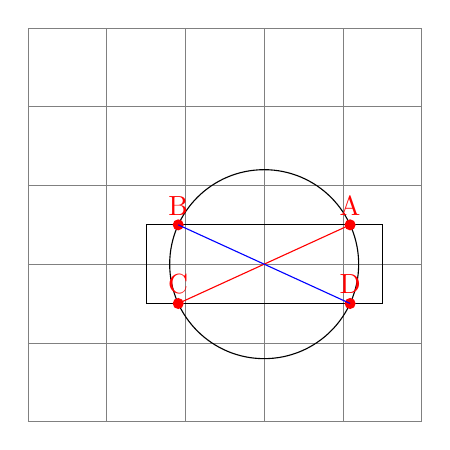
\begin{tikzpicture}
	\def\XMIN{-1}
	\def\XMAX{4}
	\def\YMIN{-1}
	\def\YMAX{4}

	%绘制辅助网格
	\draw [help lines, step=1] (\XMIN,\YMIN) grid (\XMAX,\YMAX);
	
	%使用交集
	\draw [name path=SX] (2,1) circle(1.2);
	\draw [name path=SY] (0.5,0.5) rectangle +(3,1);
	
        	\fill [red, name intersections={of=SX and SY , by={A,B,C,D}}];
        	\foreach \p in {A,B,C,D}
        		\fill [red] (\p) circle(2pt) node [above] {\p};
        	\draw [red] (A) -- (C);
        	\draw [blue] (B)  -- (D);
	
%	\fill [red, name intersections={of=SX and SY , name=SZ}];
%	\foreach \i in {1,...,4}
%		\fill [red] (SZ-\i) circle(2pt) node [above] {SZ-\i};	
%	\draw [red] (SZ-1) -- (SZ-3);
%	\draw [blue] (SZ-2) -- (SZ-4);

\end{tikzpicture}    
\end{document}
